L'elettrochimica studia fenomeni elettrici dovuti al passaggio di corrente.

Visto che ragioniamo sempre in soluzioni acquose, il passaggio di corrente provoca dei fenomeni chimici. Può accadere anche il contrario: si genera energia elettrica tramite una reazione. Tratteremo entrambi i casi.

\vspace{0.2cm}Va da ricordare che energia elettrica significa flusso di elettroni.

Le reazioni che comportano scambi di elettroni sono le ossidoriduzioni, pertanto saremo interessati a questo tipo di reazioni.

Le redox a cui siamo interessati devono essere spontanee, perché sennò avverrebbe il contrario: facendo passare la corrente in soluzione indurremo reazioni redox. Dunque qualunque reazione redox spontanea è una sorgente di energia elettrica, ossia possiamo costruire una pila a partire da reazioni redox (tutte le pile comportano reazioni redox).

Consideriamo due esempi:

\begin{figure}[H]
    \centering
    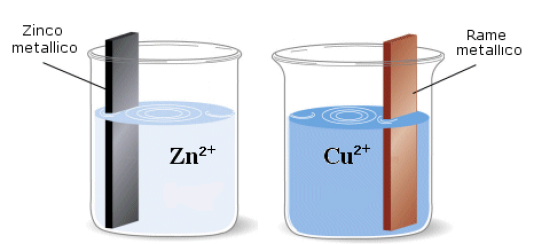
\includegraphics[width=12cm]{immagini/piastre_metalliche.png}
\end{figure}

Consideriamo dei beker contenenti acqua distillata in cui sono immersi un filo di zinco e un filo di rame. Tali sistemi sono chiamati \textbf{semicelle}.

In entrambi i casi stiamo immergendo in acqua un metallo, il quale inizia a liberare ioni. Ne segue che la lamina si caricherà di elettroni lasciati su di essa dagli ioni. Quindi la lamina, inizialmente neutra, immersa in acqua si carica negativamete e l'acqua distillata si arricchirà di ioni metallici. Quindi la soluzione inizialmente neutra si caricherà positivamente perché sta accettando cationi, mentre la lamina si caricherà negativamente perché ogni atomo che va in soluzione lascia elettroni su di essa. Poiché la lamina costituisce la parte conduttrice della semicella che estrae o immette corrente elettrica in questa viene chiamato \textbf{elettrodo} (o \textit{semielemento}).

Si crea quindi un doppio strato elettrico tra soluzione e lamina metallica, rispettivamente cariche positivamente e negativamente, e dunque si forma una differenza di potenziale. Tuttavia non siamo in grado di misurare questa d.d.p. perché per misurarla dovremmo usare un tester con cui tocchiamo la lamina con un puntale e la soluzione con l'altro, ma il puntale immerso in soluzione libererà ioni caricandosi negativamente. In conseguenza a ciò la d.d.p. letta sarebbe quella tra la lamina e il puntale immerso in soluzione, e non quella tra la lamina e la soluzione.

Come si fa?

Ci si accorge che metalli diversi hanno capacità diverse di liberare ioni in soluzione, cioè ne liberano quantità diverse. Dato che è possibile misurare gli ioni in soluzione, in quanto le soluzioni in cui sono presenti ioni conducono, si può misurare il numero di portatori di carica.

Sappiamo che la lamina di zinco, a parità di condizioni, libera molti più ioni in acqua di quanti non ne liberi la lamina di rame. Se quindi accoppiassimo questi due elettrodi in teoria sarebbero entrambi negativi, nella pratica quella di zinco è molto più negativa di quella di rame, per cui nell'istante in cui accoppiamo le due semicelle e le colleghiamo, convenzionalmente quella più negativa assumerà segno negativo e quella meno negativa segno positivo. Dunque da separati tutti i metalli liberano ioni in soluzione e sono tutti negativi, ma nel momento in cui li accoppiamo quello più negativo tra i due assumerà carica negativa e quello meno negativo carica positiva, perché il flusso di elettroni andrà sempre da quello più negativo a quello meno negativo. In questo caso il flusso di elettroni andrà dallo zinco verso il rame, cioè l'elettrodo del rame sta ricevendo elettroni, per cui sarà positivo.

Quanti elettroni liberano in soluzione?

In realtà pochi, tant'è che quando mettiamo una lamina di un metallo in acqua questa, sebbene inizi a liberare ioni, non si scioglie. Pertanto il numero di ioni liberati è limitato. Ad un certo punto però si raggiunge un equilibrio, ossia gli ioni che sono in soluzione sono positivi, ma la lamina si è caricata negativamente, quindi si genera un campo elettrico che tende a far tornare gli ioni sulla lamina. La lamina però tenderà a liberarli nuovamente, fino a quando si raggiunge un equilibrio dinamico in cui il numero di ioni liberati in soluzione è pari al numero di ioni che dalla soluzione ritornano alla lamina. Quest'equilibrio non si raggiunge velocemente perché in acqua sono presenti anche ioni $\rm H_3O^+$ dovuti all'autodissociazione dell'acqua, i quali sentono anch'essi il campo della lamina e competono con i cationi metallci per raggiungere la lamina, turbando dunque il raggiungimento dell'equilibrio.

Pertanto non è conveniente immergere lamine metalliche in acqua, in quanto difficilmente raggiungeremo un equilibrio, conviene piuttosto immergerle in soluzioni dei loro sali, in modo tale da avere già in soluzione una concentrazione di ioni metallici molto alta, di gran lunga superiore alla concentrazione di $10^{-7}$ ioni $\rm H_3O^+$ per litro dovuti all'autodissociazione dell'acqua, in modo da far sì che il turbamento dovuto a tali ioni sia irrilevante poiché la loro quantità è insignificante rispetto a quella degli ioni metallici.

\subsection{Misura della d.d.p. (pila di Daniell)}
\begin{figure}[H]
    \centering
    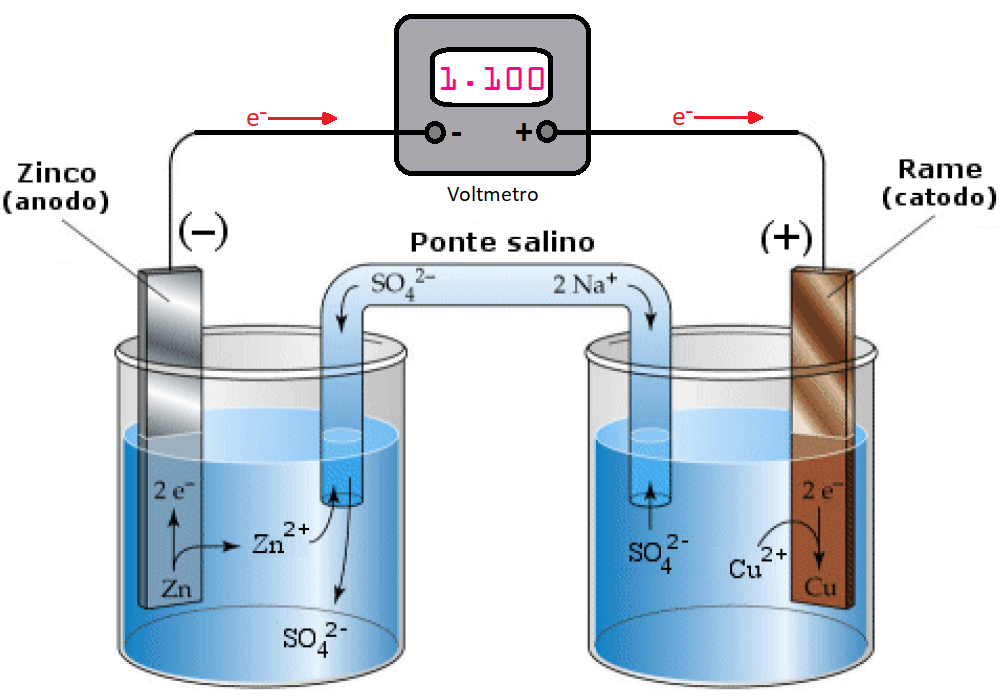
\includegraphics[width=12cm]{immagini/pila_di_Daniell.png}
\end{figure}
\begin{center}
    \hspace{0.3cm}\begin{tabular}{p{3.6cm}p{1.3cm}p{3.8cm}}
    \ce{Zn -> Zn^{2+} + 2 e^-} & & \ce{Cu^{2+} + 2e^- -> Cu}\\
    ossidazione, anodo & & riduzione, catodo
    \end{tabular}
\end{center}

Esso rappresenta il modello di pila più semplice che possiamo immmaginare.

Abbiamo una lamina di zinco immersa in una soluzione di solfato di zinco, in modo tale che quando la lamina libera ioni zinco in soluzione siano già presenti ioni di questo tipo. Ciò che accade è che lo zinco in acqua libera ioni $\rm Zn^{2+}$ e lascia due elettroni per atomo sulla lamina, che si carica negativamente.

Abbiamo poi una lamina di rame, la quale in teoria libera ioni $\rm Cu^{2+}$. Per lo stesso motivo della lamina di zinco è immersa in una soluzione di solfato di rame in cui tali ioni sono già presenti cosicché l'equilibrio si instauri velocemente.

Colleghiamo i due elettrodi. A causa del fatto che la lamina di zinco si carica più negativamente della lamina di rame perché libera in soluzione molti più ioni zinco di quanti ioni rame libera in soluzione la lamina di rame, ci saranno più elettroni sulla lamina di zinco che su quella di rame e quindi gli elettroni fluiranno dalla prima alla seconda.

Per chiudere il circuito però dobbiamo collegare anche le soluzioni. Infatti nelle condizioni in cui di trova adesso
il sistema abbiamo un'abbondanza di elettroni sulla lamina che genera il flusso, ma se consumiamo gli elettroni su di essa, questa tenderà a ripristinarli liberando in soluzione altri ioni zinco, ossia man mano che consumiamo elettroni la lamina tende a sciogliersi, poiché i suoi atomi passano da Zn a $\rm Zn^{2+}$.

Dall'altra parte la lamina su cui arrivano gli elettroni vedrà una reazione diversa: gli ioni rame del solfato di rame acquistano gli elettroni e si riducono passando da $\rm Cu^{2+}$ a $\rm Cu^0$:

$$(-) \; \ce{Zn <--> Zn^{2+}(aq) + 2e^-} \qquad (+) \; \ce{ Cu^{2+}(aq) + 2e^- <--> Cu}$$

Quindi su un elettrodo abbiamo l'ossidazione dello zinco, sull'altro la riduzione del rame. Cosa succede alle soluzioni appena avviene ciò?

A sinistra arrivano ioni zinco, e la soluzione inizialmente neutra a causa degli ioni $\rm Zn^{2+}$ in eccesso si carica positivamente. Al contrario a destra alcuni ioni rameici si depositano sulla lamina di rame e la soluzione da neutra passa ad avere eccesso di ioni $\rm SO_4^{2-}$ e quindi si carica negativamente.

La conseguenza del fatto che le soluzioni si siano caricate è che il processo di passaggio di elettroni non avviene, in quanto non viene garantita la neutralità delle soluzioni.

\E quindi necessario collegare le due soluzioni, o in termini fisici è necessario chiudere il circuito. Per chiudere il circuito di due soluzioni serve un'altra soluzione.

Colleghiamo le due soluzioni con un tubo di vetro all'interno del quale c'è una gelatina formata dall'alga agar, la quale essiccata e ridotta in polvere impastata con l'acqua dà luogo ad un gel. Dunque prepariamo una gelatina fatta di questa polvere ottenuta dall'alga secca, nella quale aggiungiamo un sale. Nel caso specifico aggiungiamo cloruro di potassio. Non tutti i sali vanno bene (vedremo perché).

La gelatina non è molto liquida, anzi è molto faticoso farla entrare nel tubo di vetro. Ciò fa sì che non cada nella soluzione.

Riprendiamo ciò che succede nelle soluzioni. A sinistra lo zinco si scioglie e libera ioni zinco. Il cloruro di potassio sente il campo elettrico degli ioni zinco e libera ioni $\rm Cl^-$ , quindi negativi, che vanno a neutralizzare l'eccesso di $\rm Zn^{2+}$. A destra invece perdiamo ioni $\rm Cu^{2+}$ perché vanno a depositarsi sulla lamina di rame, dando luogo ad eccesso di $\rm SO_4^{2-}$. Lo ione $\rm K^+$ del cloruro di potassio sente questo campo elettrico, per cui si libera per diffondersi nella soluzione di solfato di rame, neutralizzando la carica dovuta all'eccesso di $\rm SO_4^{2-}$. In questo modo istante per istante viene assicurata l'elettro-neutralità delle due soluzioni, cosa che permette alla reazione di riprendere, facendo sciogliere la lamina di zinco e facendo ispessire quella di rame.

Ci sarà così un flusso di elettroni, quindi abbiamo una pila formata semplicemente da due soluzioni, due metalli diversi ed un ponte salino. In particolare questa dell'esempio dà una d.d.p. di 1.1 V.

Qualunque metallo in acqua libera ioni, pertanto con questo metodo possiamo fare un numero infinito di pile accoppiando i vari metalli o anche modificando le concentrazioni delle soluzioni.

La reazione che avviene nel nostro esempio è

$$\ce{Zn + Cu^{2+}(aq) <--> Zn^{2+}(aq) + Cu}$$

Lo zinco metallico della lamina di rame e gli ioni $\rm Cu^{2+}$ della soluzione del solfato di rame instaurano un equilibrio in cui otteniamo ioni zinco $\rm Zn^{2+}$ e gli ioni $\rm Cu^{2+}$ diventano Cu, depositandosi sulla lamina.

Abbiamo quindi l'ossidazione dello zinco e la riduzione del rame.

L'elettrodo negativo dello zinco si chiama \textbf{anodo}, quello positivo del rame si chiama \textbf{catodo}.

Attenzione! In questo fenomeno stiamo sviluppando un flusso di elettroni e quindi generiamo energia elettrica con una reazione chimica. Nel fenomeno opposto, in cui induciamo reazioni chimiche tramite energia elettrica, i nomi degli elettrodi si invertono: anodo positivo e catodo negativo. Per non sbagliare basta ricordare che le riduzioni avverranno sempre al catodo, sia che stiamo osservando una pila che un'elettrolisi.

Se la differenza di energia per 1 C di carica è di 1 J, il potenziale della cella sarà di 1 V: $1 V=\frac{1J}{C}$.

Cerchiamo adesso di quantificare questo fenomeno. Stiamo discutendo di reazioni spontanee: immergiamo gli elettrodi nelle due soluzioni, colleghiamo gli elettrodi, mettiamo il ponte salino e stiamo a guardare, e il sistema genera energia elettrica. Se la reazione è spontanea, il lavoro è detto utile ed è uguale aall'opposto della variazione di energia libera. Nel nostro caso il lavoro utile è il lavoro elettrico, il quale è dato dalla carica $q$ misurata in Coulomb per la d.d.p. $E$, e a sua volta la carica è data dal numero di elettroni scambiati $n$ per la costante di Faraday $F$:

$$L_{\text{utile}}=- \Delta G; \; L_{\text{utile}}=L_{\text{elettrico}}=q_c \times E=nFE \implies \Delta G = -nFE$$

con $q_c$ carica, $E$ d.d.p.\, $1F=6.023 \cdot 10^{23} \cdot 1.6023 \cdot 10^{-19} \, C = 96485 \, C$

La costante di Faraday $F$ si ottiene moltiplicando la carica dell'elettrone per il numero di avogadro, cioè è la carica di una mole di elettroni.

Consideriamo una generica reazione

$$\ce{\alpha A + \beta B <--> \gamma C + \delta D}$$

con $\alpha, \; \beta, \; \gamma$ e $\delta$ coefficienti stechiometrici.

Studiando la legge di azione delle masse abbiamo visto che

$$\Delta G = \Delta G^0 + RT\ln k \quad \text{con }k \text{ costante di equilibrio}$$

All'equilibrio la variazione di energia libera deve essere zero:

$$\Delta G=0 \implies \Delta G^0= -RT \ln k$$

Eguagliando allora le due definizioni di $\Delta G$ avremo che

$$\Delta G =  -RT \ln k_{eq} + RT \ln \frac{a_C^{\gamma} \, a_D^{\delta}}{a_A^{\alpha} \, a_B^{\beta}}=-nFE$$

Va da notare che nelle costanti non compaiono le concentrazioni: al loro posto abbiamo l'\textbf{attività} $a$. Essa è un'unità di misura molto più precisa delle concentrazioni perché se mettiamo degli ioni in soluzione troveremo un valore per la concentrazione, ma non siamo sicuri che questi ioni siano talmente vicini da formare coppie ioniche e pertanto sottrarsi all'influenza di un possibile campo elettrico, in quanto si comporterebbero come se fossero un'unica entità. L'attività tiene conto di questo fatto, quindi ci dice in maniera più precisa quante speci chimiche abbiamo in soluzione.

L'attività delle speci pure è considerata pari a 1. Ciò è molto utile. Ad esempio nella pila che abbiamo visto la lamina di zinco libera ioni zinco, per cui abbiamo la forma ossidata che è $\rm Zn^{2+}$ e la forma ridotta che è Zn. Quest'ultimo è un metallo puro, quindi la sua attività è pari a 1. D'altra parte una lamina metallica immersa in acqua non ha concentrazione.

Esplicitiamo $E$ dalla precedente equazione:

$$E=\frac{RT}{nF}\ln k_{eq} - \frac{RT}{nF}\ln \frac{a_C^{\gamma} \, a_D^{\delta}}{a_A^{\alpha} \, a_B^{\beta}}$$

Se la temperatura è costante il primo termine sarà pari ad una costante $E^0$:

$$E= E^0 + \frac{RT}{nF}\ln \frac{a_A^{\alpha} \, a_B^{\beta}}{a_C^{\gamma} \, a_D^{\delta}} \quad \textbf{Equazione di Nernst}$$

Nota: siccome abbiamo cambiato il segno del logaritmo, adesso al numeratore abbiamo i reagenti e al denominatore i prodotti.

Tale equazione permette di calcolare la d.d.p. di una pila. Infatti in essa compaiono 4 attività che sono quelle dei 4 termini che compaiono nella redox della pila ($\rm Zn, \; Zn^{2+}, \; Cu^{2+}$ e $\rm Cu$).

Se poniamo
$$R=8.314 \, J/mol\,K, \quad \ln x = 2.303 \log x, \quad F=96485 \, C, \quad T=298 \,K$$

L'equazione diventa

$$E = E^0 + \frac{0.059}{n}\log \frac{a_A^{\alpha} \, a_B^{\beta}}{a_C^{\gamma} \, a_D^{\delta}}$$

$n$ resta tale perché dipende da quanti elettroni genera quella reazione.

\vspace{0.2cm}Per un generico elettrodo vale
$$\ce{\alpha ox + ne^- <--> \beta rid}$$

La forma ossidata dà la forma ridotta (se ad essa diamo un certo numero di elettroni). $\alpha$ e $\beta$ sono i coefficienti stechiometrici.

Nel caso dei metalli la reazione è
$$\ce{\alpha M^{n+} + ne^- <--> \beta M}$$

Quindi per un elettrodo le speci sono due: la forma ossidata $\rm M^{n+}$ e la forma ridotta M. L'equazione di Nernst allora diventa

$$E = E^0 + \frac{0.059}{n}\log \frac{a_{ox}^{\alpha}}{a_{rid}^{\beta}}$$

\vspace{0.2cm}Per definizione l'attività dei solidi puri è pari a 1, quindi $a_{rid}=1$. Pertanto per un singolo elettrodo avremo:

$$E = E^0 + \frac{0.059}{n}\log a{(\text{M}^{n+})}^{\alpha}$$

dove $n$ è il numero di elettroni scambiati, $a(\text{M}^{n+})$ è la concentrazione del catione in soluzione.

In questo modo calcoliamo la d.d.p. di un elettrodo.

Attenzione! Non abbiamo ancora calcolato $E^0$.